\documentclass[3p,sort&compress,11pt,fleqn]{elsarticle}
\usepackage{setspace,tikz,float,booktabs,amsmath,amssymb,mathpazo,siunitx,structmech}
\usetikzlibrary{shapes,arrows.meta}
%\tikzset{>={Latex[width=2mm,length=2mm]},base/.style={rectangle,rounded corners,draw=black,minimum width=1cm,minimum height=1cm,text centered,font=\sffamily}
%}
\bibliographystyle{elsarticle-num-names}
\journal{IJNME}
\newcommand*{\figref}[1]{Fig.~\ref{#1}}
\newcommand*{\eqsref}[1]{Eq.~(\ref{#1})}
\newcommand*{\tabref}[1]{Table~\ref{#1}}
\newcommand*{\class}[1]{\texttt{#1}}
%\newcommand*{\mathbold}[1]{\mathbf{#1}}
\newcommand*{\mT}{\mathrm{T}}
\newcommand*{\md}[1]{\mathrm{d}#1}
\newcommand*{\pfrac}[2]{\dfrac{\partial#1}{\partial#2}}
\onehalfspacing
\begin{document}
\begin{abstract}
This work discusses the finite element formulation based on a six-field variational principle that incorporates the consistent couple stress theory. The corresponding solving procedure that covers both linear and nonlienar materials is derived. With the implemented membrane elements, the numerical experiments are conducted to investigate the performance of the in-plane drilling degrees of freedom introduced by the consistent couple stress theory.
\end{abstract}
\begin{keyword}
mixed formulation\sep
couple stress theory\sep
size dependence
\end{keyword}
\begin{frontmatter}
\title{Mixed formulation of finite elements based on couple stress theory}
\author[]{T.~L.~Chang\corref{tlc}}\ead{tlcfem@gmail.com}
%\cortext[tlc]{corresponding author}
\address{Department of Civil and Natural Resources Engineering, University of Canterbury, Christchurch, New Zealand, 8041.}
\end{frontmatter}
\section{Introduction}
The Cauchy continuum mechanics has received wide recognition over the years and becomes the standard framework for many engineering disciplines. For simple, idealised problems, analytical solutions can be constructed \citep[see, e.g.,][]{Timoshenko2010} with proper assumptions. The Cauchy theory also provides theoretical basis for the extensively used finite element methods. However, due to the lack of proper measure of rotation/curvature (and its force/stress conjugate), certain difficulties are encountered in problems involving beams, plates, shells, etc. Besides, the Cauchy theory is incapable of describing the size effect, which is frequently seen in many materials at various scales (from nano to macro) and plays a vital role in fracture mechanics \citep{Bazant1984}.

The consistent couple stress theory \citep{Hadjesfandiari2011} provides a promising tool to address the aforementioned shortcomings of the Cauchy theory.

Recent research work on membrane elements with in-plane drilling degrees of freedom can be seen in the review by \citet{Boutagouga2020}. For reviews on theoretical developments and experimental investigations regarding couple stress theory, interested authors can refer to the work by \citet{Pedgaonkar2021} and the references therein.

The drilling degree of freedom defined within Cauchy theory shows significant size effect, which limits its application in modelling problems involving both membrane and beam elements \citep{Chang2020}.

This paper is organised as follows. The consistent couple stress theory is briefly reviewed by summarising key equations and quantities that are later used in finite element formulation. Based on this theory, a general mixed variational principle involving six independent fields are derived. Two elements couple stress triangle and quadrilateral elements are developed after formulating system of linear equations. With the proposed elements, the performance of the drilling degree of freedom is further investigated by conducting numerical experiments.
\section{The Couple Stress Theory}
Details of the adopted consistent couple stress theory can be seen in the work by \citet{Hadjesfandiari2011}. Here a brief summary of all necessary expressions utilised in finite element formulation is presented.
\subsection{Kinematics}
Within the infinitesimal strain framework, the couple stress theory \citep{Hadjesfandiari2011} accounts for both symmetric and skew--symmetric parts of displacement gradient in kinematics, that is
\begin{gather}\label{eq:varepsilon}
\varepsilon_{ij}=\dfrac{1}{2}\left(u_{i,j}+u_{j,i}\right),\\
\omega_{ij}=\dfrac{1}{2}\left(u_{i,j}-u_{j,i}\right),
\end{gather}
where $u_i$ is the displacement field, $\varepsilon_{ij}$ is the infinitesimal strain tensor, $\omega_{ij}$ is the skew--symmetric strain tensor that can be equivalently represented by the rotation vector $\theta_i$,
\begin{gather}\label{eq:theta}
\theta_i=\dfrac{1}{2}\epsilon_{ijk}\omega_{kj}=\dfrac{1}{2}\epsilon_{ijk}u_{k,j},
\end{gather}
where $\epsilon_{ijk}$ is the Levi--Civita (permutation) symbol. By utilising $\theta_i$, the mean curvature vector $\kappa_i$ is defined as
\begin{gather}\label{eq:kappa}
\kappa_i=\dfrac{1}{2}\epsilon_{ijk}\theta_{k,j},
\end{gather}
which can be further expressed in terms of $u_i$ so that
\begin{gather}
\kappa_i=\dfrac{1}{4}\left(u_{j,ij}-u_{i,jj}\right).
\end{gather}
The engineering mean curvature $k_i$ can be defined accordingly to be
\begin{gather}
k_i=-2\kappa_i.
\end{gather}
\subsection{Equilibrium}
The total stress tensor consists of two parts, namely the conventional symmetric stress tensor $\sigma_{ij}$ and the additional skew--symmetric couple stress tensor $\mu_{ij}$. Compared to the original literature \citep{Hadjesfandiari2011}, here a slightly different notation is used for brevity.

The couple stress vector $\mu_i$ dual to $\mu_{ij}$ can be defined as
\begin{gather}
\mu_{ji}=\epsilon_{ijk}\mu_k.
\end{gather}
It is found that $\mu_i$ is the energetic conjugate to engineering mean curvature $k_i$.

The corresponding equilibrium equation can be shown as
\begin{gather}\label{eq:equilibrium}
\sigma_{ji,j}+\dfrac{1}{2}\left(\mu_{j,ij}-\mu_{i,jj}\right)+f_i=0,
\end{gather}
where $f_i$ is the body force field.
\subsection{Linear Elasticity}
The stored energy function $W$ can be defined as a function of $\varepsilon_{ij}$ and $\kappa_i$ such that
\begin{gather}
W\left(\varepsilon_{ij},\kappa_i\right)=\dfrac{1}{2}\lambda\varepsilon_{ii}\varepsilon_{jj}+\mu\varepsilon_{ij}\varepsilon_{ij}+8\eta\kappa_i\kappa_i,
\end{gather}
where $\lambda$ and $\mu$ are Lam\'{e} constants, $\eta$ is the additional material constant. The corresponding constitutive relations for linear elasticity can then be derived to be
\begin{gather}\label{eq:constitutive_couple}
\mu_i=-8\eta\kappa_i=4\eta{}k_i,\\
\sigma_{ij}=\lambda\delta_{ij}\varepsilon_{kk}+2\mu\varepsilon_{ij},
\end{gather}
where $\delta_{ij}$ is the Kronecker delta. The additional constant $\eta$ can be related to shear modulus $\mu$ by the characteristic length $l$ according to the following expression,
\begin{gather}
\eta=l^2\mu.
\end{gather}

Given that in this work $\sigma_{ij}$ is assumed to be symmetric, without loss of generality, the variation of $W$ can be expressed as
\begin{gather}\label{eq:potential_energy}
\delta{}W\left(\varepsilon_{ij},\kappa_i\right)=\bar{\sigma}_{ij}\delta\varepsilon_{ij}-2\bar{\mu}_{i}\delta\kappa_i,
\end{gather}
or
\begin{gather}
\delta{}W\left(\varepsilon_{ij},k_i\right)=\bar{\sigma}_{ij}\delta\varepsilon_{ij}+\bar{\mu}_{i}\delta{}k_i,
\end{gather}
with $\bar{\sigma}_{ij}$ and $\bar{\mu}_{i}$ denoting stress and couple stress tensors obtained from typical strain driven constitutive model. For linear elasticity, they are simply
\begin{gather*}
\bar{\sigma}_{ij}=\sigma_{ij},\qquad\bar{\mu}_{i}=\mu_{i}.
\end{gather*}
\subsection{Remarks}
It could be noted that $C^1$ continuity is required by the displacement field $u_i$ due to the presence of the second order derivatives in $\kappa_i$. Shape functions based on such as NURBS \citep[see][]{Dargush2021} that support $C^1$ continuity can be adopted to construct properly finite elements. Alternatively, $\theta_i$ can be treated as an independent field and the corresponding kinematic equations can be introduced into the functional via the method of Lagrangian multiplier, applications of which can be seen for example in the work by \citet{Darrall2013,Deng2016,Pedgaonkar2021}. Further discussions of such a consistent couple stress theory can be also seen in the work by \citet{Hadjesfandiari2016}.
\section{A Six--Field Mixed Framework}
In this section, the variational theorem developed by \citet{Darrall2013} is further extended to a more general form which resembles the Hu--Washizu variational theorem in the classic Cauchy theory.

By assuming the essential boundary conditions can be satisfied by proper construction, in absence of body force and surface force/moment traction, the total potential energy functional over an arbitrary domain $V$ can be simply expressed as
\begin{gather}
\varPi\left(\varepsilon_{ij},\kappa_i\right)=\int_VW~\md{V}
\end{gather}
where $W\left(\varepsilon_{ij},\kappa_i\right)$ is defined in \eqsref{eq:potential_energy} for linear elastic material. Since $\varepsilon_{ij}\left(u_i\right)$ and $\kappa_i\left(u_i\right)$ are functions of $u_i$, $u_i$ is the only independent field in the above functional.

Now consider the case in which $u_i$, $\theta_i$, $\varepsilon_{ij}$, and $\kappa_i$ are all treated as independent fields, the kinematic equations \eqsref{eq:varepsilon}, \eqsref{eq:kappa} and \eqsref{eq:theta} need to be satisfied in a weak form. By introducing three Lagrangian multipliers $\alpha_{ij}$, $\beta_i$ and $\gamma_i$, those equations can be appended to the above functional so that
\begin{multline}
\varPi\left(u_i,\theta_i,\varepsilon_{ij},\kappa_i,\alpha_{ij},\beta_i,\gamma_i\right)=\int_VW~\md{V}
+\int_V\alpha_{ij}\left(\varepsilon_{ij}-\dfrac{1}{2}\left(u_{i,j}+u_{j,i}\right)\right)~\md{V}\\
+\int_V\beta_i\left(\kappa_i-\dfrac{1}{2}\epsilon_{ijk}\theta_{k,j}\right)~\md{V}
+\int_V\gamma_i\left(\theta_i-\dfrac{1}{2}\epsilon_{ijk}u_{k,j}\right)~\md{V}.
\end{multline}
Taking the first variation leads to
\begin{gather}\label{eq:variation}
\begin{split}
\delta\varPi&=
\int_V\bar{\sigma}_{ij}\delta\varepsilon_{ij}~\md{V}
-\int_V2\bar{\mu}_{i}\delta\kappa_i~\md{V}\\&
+\int_V\delta{}\alpha_{ij}\left(\varepsilon_{ij}-\dfrac{1}{2}\left(u_{i,j}+u_{j,i}\right)\right)~\md{V}
+\int_V\alpha_{ij}\left(\delta{}\varepsilon_{ij}-\dfrac{1}{2}\left(\delta{}u_{i,j}+\delta{}u_{j,i}\right)\right)~\md{V}\\&
+\int_V\delta{}\beta_i\left(\kappa_i-\dfrac{1}{2}\epsilon_{ijk}\theta_{k,j}\right)~\md{V}
+\int_V\beta_i\left(\delta{}\kappa_i-\dfrac{1}{2}\epsilon_{ijk}\delta{}\theta_{k,j}\right)~\md{V}\\&
+\int_V\delta{}\gamma_i\left(\theta_i-\dfrac{1}{2}\epsilon_{ijk}u_{k,j}\right)~\md{V}
+\int_V\gamma_i\left(\delta{}\theta_i-\dfrac{1}{2}\epsilon_{ijk}\delta{}u_{k,j}\right)~\md{V}.
\end{split}
\end{gather}
By performing integration by parts and applying the divergence theorem, one can find
\begin{gather}
-\dfrac{1}{2}\int_V\alpha_{ij}\left(\delta{}u_{i,j}+\delta{}u_{j,i}\right)~\md{V}=\int_V\dfrac{\alpha_{ij,j}+\alpha_{ji,j}}{2}\delta{}u_i~\md{V}-\int_S\dfrac{\alpha_{ij}+\alpha_{ji}}{2}n_j\delta{}u_i~\md{S},\\
-\dfrac{1}{2}\int_V\epsilon_{ijk}\beta_i\delta\theta_{k,j}~\md{V}=\dfrac{1}{2}\int_V\epsilon_{ijk}\beta_{i,j}\delta\theta_k~\md{V}-\dfrac{1}{2}\int_S\epsilon_{ijk}\beta_in_j\delta\theta_k~\md{S},\\
-\dfrac{1}{2}\int_V\epsilon_{ijk}\gamma_i\delta{}u_{k,j}~\md{V}=\dfrac{1}{2}\int_V\epsilon_{ijk}\gamma_{i,j}\delta{}u_k~\md{V}-\dfrac{1}{2}\int_S\epsilon_{ijk}\gamma_in_j\delta{}u_k~\md{S}.
\end{gather}
Here $S$ is not further refined for simplicity.

Inserting the above expressions back to \eqsref{eq:variation} gives
\begin{gather}
\begin{split}
\delta\varPi&=
\int_V\bar{\sigma}_{ij}\delta\varepsilon_{ij}~\md{V}+\int_V\alpha_{ij}\delta{}\varepsilon_{ij}~\md{V}
-\int_V2\bar{\mu}_{i}\delta\kappa_i~\md{V}+\int_V\beta_i\delta{}\kappa_i~\md{V}\\&
+\int_V\delta{}\alpha_{ij}\left(\varepsilon_{ij}-\dfrac{1}{2}\left(u_{i,j}+u_{j,i}\right)\right)~\md{V}
+\int_V\delta{}\beta_i\left(\kappa_i-\dfrac{1}{2}\epsilon_{ijk}\theta_{k,j}\right)~\md{V}\\&
+\int_V\delta{}\gamma_i\left(\theta_i-\dfrac{1}{2}\epsilon_{ijk}u_{k,j}\right)~\md{V}
+\int_V\dfrac{\alpha_{ij,j}+\alpha_{ji,j}}{2}\delta{}u_i~\md{V}
+\dfrac{1}{2}\int_V\epsilon_{ijk}\gamma_{i,j}\delta{}u_k~\md{V}\\&
+\int_V\gamma_i\delta{}\theta_i~\md{V}+\dfrac{1}{2}\int_V\epsilon_{ijk}\beta_{i,j}\delta\theta_k~\md{V}-\dfrac{1}{2}\int_S\epsilon_{ijk}\beta_in_j\delta\theta_k~\md{S}\\&
-\int_S\dfrac{\alpha_{ij}+\alpha_{ji}}{2}n_j\delta{}u_i~\md{S}-\dfrac{1}{2}\int_S\epsilon_{ijk}\gamma_in_j\delta{}u_k~\md{S}.
\end{split}
\end{gather}

Since the variations $\delta{}u_i$, $\delta{}\theta_i$, $\delta{}\varepsilon_{ij}$, $\delta{}\kappa_i$, $\delta{}\alpha_{ij}$, $\delta{}\beta_i$ and $\delta{}\gamma_i$ are arbitrary, the stationary condition requires the following equations involving Lagrangian multipliers to hold.
\begin{gather}
%\left\{\begin{array}{l}
\bar{\sigma}_{ij}+\alpha_{ij}=0,\quad
-2\bar{\mu}_i+\beta_i=0,\quad
\alpha_{kj,j}+\alpha_{jk,j}+\epsilon_{ijk}\gamma_{i,j}=0,\quad
\gamma_k+\dfrac{1}{2}\epsilon_{ijk}\beta_{i,j}=0.
%\end{array}\right.
\end{gather}
It can be identified that $\alpha_{ij}=-\sigma_{ij}$, $\beta_i=2\mu_i$ and $\gamma_i=\epsilon_{ijk}\mu_{k,j}$ with $\sigma_{ij}$ and $\mu_i$ be independent fields. The third equation is essentially
\begin{gather*}
\begin{split}
0=\left(\alpha_{kj}+\alpha_{jk}\right)_{,j}+\epsilon_{ijk}\epsilon_{imn}\mu_{m,nj}=\left(\alpha_{ji}+\alpha_{ij}\right)_{,j}+\left(\mu_{j,i}-\mu_{i,j}\right)_{,j},
\end{split}
\end{gather*}
which is the stress equilibrium \eqsref{eq:equilibrium} in absence of body force $f_i$.

The functional in its general form is then
\begin{multline}
\varPi\left(u_i,\theta_i,\varepsilon_{ij},\sigma_{ij},\kappa_i,\mu_i\right)=\int_VW~\md{V}
-\int_V\sigma_{ij}\left(\varepsilon_{ij}-\dfrac{1}{2}\left(u_{i,j}+u_{j,i}\right)\right)~\md{V}\\
+\int_V2\mu_i\left(\kappa_i-\dfrac{1}{2}\epsilon_{ijk}\theta_{k,j}\right)~\md{V}
+\int_V\epsilon_{imn}\mu_{n,m}\left(\theta_i-\dfrac{1}{2}\epsilon_{ijk}u_{k,j}\right)~\md{V}.
\end{multline}
It shall be noted that all boundary terms are omitted for brevity. In vector/matrix form, it can also be written as
\begin{multline}\label{eq:functional}
\varPi\left(\mathbold{u},\mathbold{\theta},\mathbold{\varepsilon},\mathbold{\sigma},\mathbold{\kappa},\mathbold{\mu}\right)=\int_VW~\md{V}
+\int_V\mathbold{\sigma}^\mT\left(\nabla^s\mathbold{u}-\mathbold{\varepsilon}\right)~\md{V}\\
+\int_V2\mathbold{\mu}^\mT\left(\mathbold{\kappa}-\dfrac{1}{2}\nabla\times\mathbold{\theta}\right)~\md{V}
+\int_V\left(\nabla\times\mathbold{\mu}\right)^\mT\left(\mathbold{\theta}-\dfrac{1}{2}\nabla\times\mathbold{u}\right)~\md{V}.
\end{multline}
The symbol $\nabla^s\mathbold{u}$ is used to denote the result of $\left(u_{i,j}+u_{j,i}\right)/2$ expressed in Voigt form.

It occupies a form similar to that of the functional used in the Hu--Washizu principle. Fields $\mathbold{u}$, $\mathbold{\theta}$ and $\mathbold{\mu}$ require $C^0$ continuity, while $\mathbold{\kappa}$, $\mathbold{\varepsilon}$ and $\mathbold{\sigma}$ can be constant fields. Starting from \eqsref{eq:functional}, various levels of simplifications can be conducted to derive both mixed--type and hybrid--type finite elements. For example, any of \eqsref{eq:varepsilon}, \eqsref{eq:kappa} and \eqsref{eq:theta} can be satisfied in strong forms thus the corresponding terms can be omitted from the functional. The mixed functional used by \citet{Darrall2013}, which is
\begin{gather}
\varPi\left(\mathbold{u},\mathbold{\theta},\mathbold{\mu}\right)=\int_VW~\md{V}
+\int_V\left(\nabla\times\mathbold{\mu}\right)^\mT\left(\mathbold{\theta}-\dfrac{1}{2}\nabla\times\mathbold{u}\right)~\md{V}+\varPi_{b.t.}.
\end{gather}
can be obtained by enforcing \eqsref{eq:varepsilon} and \eqsref{eq:kappa} in strong forms. Besides, by considering \eqsref{eq:varepsilon} only, another functional can be obtained.
\begin{multline}
\varPi\left(\mathbold{u},\mathbold{\theta},\mathbold{\kappa},\mathbold{\mu}\right)=\int_VW~\md{V}
+\int_V2\mathbold{\mu}^\mT\left(\mathbold{\kappa}-\dfrac{1}{2}\nabla\times\mathbold{\theta}\right)~\md{V}\\
+\int_V\left(\nabla\times\mathbold{\mu}\right)^\mT\left(\mathbold{\theta}-\dfrac{1}{2}\nabla\times\mathbold{u}\right)~\md{V}+\varPi_{b.t.}.
\end{multline}
One can also apply divergence theorem to terms involving derivatives to convert between volume and surface integrals.

If, instead of $\mathbold{\kappa}$, engineering mean curvature $\mathbold{k}$ is used, an equivalent form can be derived following the same procedure.
\begin{multline}\label{eq:functional2}
\varPi\left(\mathbold{u},\mathbold{\theta},\mathbold{\varepsilon},\mathbold{\sigma},\mathbold{k},\mathbold{\mu}\right)=\int_VW~\md{V}
+\int_V\mathbold{\sigma}^\mT\left(\nabla^s\mathbold{u}-\mathbold{\varepsilon}\right)~\md{V}\\
-\int_V\mathbold{\mu}^\mT\left(\mathbold{k}+\nabla\times\mathbold{\theta}\right)~\md{V}
+\int_V\left(\nabla\times\mathbold{\mu}\right)^\mT\left(\mathbold{\theta}-\dfrac{1}{2}\nabla\times\mathbold{u}\right)~\md{V}.
\end{multline}
As can be predicted, the difference is solely the term $\displaystyle\int_V2\mathbold{\mu}^\mT\mathbold{\kappa}~\md{V}=-\int_V\mathbold{\mu}^\mT\mathbold{k}~\md{V}$.
\section{Finite Element Formulation}
In this section, the linear equation system of the aforementioned general six--field variational principle \eqsref{eq:functional} is derived. Since there is no other local residual apart from the one due to potential inelastic constitutive models, a locally iterative algorithm is not required. The final elemental stiffness may possess a form similar to that of conventional displacement based elements.
\subsection{Linear System}
Let six fields be discretized as follows.
\begin{gather}
\mathbold{u}=\mathbold{\phi}_\mathbold{u}\mathbold{p},\quad
\mathbold{\theta}=\mathbold{\phi}_\mathbold{\theta}\mathbold{q},\quad
\mathbold{\kappa}=\mathbold{\phi}_\mathbold{\kappa}\mathbold{r},\quad
\mathbold{\mu}=\mathbold{\phi}_\mathbold{\mu}\mathbold{s},\quad
\mathbold{\varepsilon}=\mathbold{\phi}_\mathbold{\varepsilon}\mathbold{\beta},\quad
\mathbold{\sigma}=\mathbold{\phi}_\mathbold{\sigma}\mathbold{\alpha}.
\end{gather}
Then, naturally, $\nabla^s\mathbold{u}=\mathbold{L}\mathbold{\phi}_\mathbold{u}\mathbold{p}$ where $\mathbold{L}$ is the differential operator which can be expressed as
\begin{gather}
\mathbold{L}=\begin{bmatrix}
\pfrac{}{x}&\cdot&\cdot&\pfrac{}{y}&\cdot&\pfrac{}{z}\\[4mm]
\cdot&\pfrac{}{y}&\cdot&\pfrac{}{x}&\pfrac{}{z}&\cdot\\[4mm]
\cdot&\cdot&\pfrac{}{z}&\cdot&\pfrac{}{y}&\pfrac{}{x}
\end{bmatrix}^\mT
\end{gather}
in 3D space. Similarly, the curl operator can be expressed as $\dfrac{1}{2}\nabla\times\left(\cdot\right)=\mathbold{J}\left(\cdot\right)$ with
\begin{gather}
\mathbold{J}=\dfrac{1}{2}\begin{bmatrix}
\cdot&-\pfrac{}{z}&\pfrac{}{y}\\[4mm]
\pfrac{}{z}&\cdot&-\pfrac{}{x}\\[4mm]
-\pfrac{}{y}&\pfrac{}{x}&\cdot
\end{bmatrix}.
\end{gather}

Now the functional can be rewritten as
\begin{multline}\label{eq:functional_new}
\varPi\left(\mathbold{p},\mathbold{q},\mathbold{r},\mathbold{s},\mathbold{\beta},\mathbold{\alpha}\right)=\int_VW~\md{V}
+\int_V\mathbold{\alpha}^\mT\mathbold{\phi}_\mathbold{\sigma}^\mT\left(\mathbold{L}\mathbold{\phi}_\mathbold{u}\mathbold{p}-\mathbold{\phi}_\mathbold{\varepsilon}\mathbold{\beta}\right)~\md{V}\\
+\int_V2\mathbold{s}^\mT\mathbold{\phi}_\mathbold{\mu}^\mT\left(\mathbold{\phi}_\mathbold{\kappa}\mathbold{r}-\mathbold{J}\mathbold{\phi}_\mathbold{\theta}\mathbold{q}\right)~\md{V}
+\int_V2\mathbold{s}^\mT\left(\mathbold{J}\mathbold{\phi}_\mathbold{\mu}\right)^\mT\left(\mathbold{\phi}_\mathbold{\theta}\mathbold{q}-\mathbold{J}\mathbold{\phi}_\mathbold{u}\mathbold{p}\right)~\md{V}.
\end{multline}

Taking variations leads to the following system of equations.
\begin{gather}\label{eq:stationary}
\left\{
\begin{array}{lll}
\dfrac{\delta\varPi}{\delta{}\mathbold{p}}=\mathbold{0}&\longrightarrow&\displaystyle\int_V\left(\mathbold{L}\mathbold{\phi}_\mathbold{u}\right)^\mT\mathbold{\phi}_\mathbold{\sigma}\mathbold{\alpha}-2\left(\mathbold{J}\mathbold{\phi}_\mathbold{u}\right)^\mT\left(\mathbold{J}\mathbold{\phi}_\mathbold{\mu}\right)\mathbold{s}~\md{V}=\mathbold{R}_\mathbold{u},\\[4mm]
\dfrac{\delta\varPi}{\delta{}\mathbold{q}}=\mathbold{0}&\longrightarrow&\displaystyle\int_V2\left(\mathbold{\phi}_\mathbold{\theta}^\mT\mathbold{J}\mathbold{\phi}_\mathbold{\mu}-\left(\mathbold{J}\mathbold{\phi}_\mathbold{\theta}\right)^\mT\mathbold{\phi}_\mathbold{\mu}\right)\mathbold{s}~\md{V}=\mathbold{R}_\mathbold{\theta},\\[4mm]
\dfrac{\delta\varPi}{\delta{}\mathbold{r}}=\mathbold{0}&\longrightarrow&\displaystyle\int_V\mathbold{\phi}_\mathbold{\kappa}^\mT{}W_\mathbold{\kappa}+2\mathbold{\phi}_\mathbold{\kappa}^\mT\mathbold{\phi}_\mathbold{\mu}\mathbold{s}~\md{V}=\mathbold{0},\\[4mm]
\dfrac{\delta\varPi}{\delta{}\mathbold{s}}=\mathbold{0}&\longrightarrow&\displaystyle
\int_V2\left(\left(\mathbold{J}\mathbold{\phi}_\mathbold{\mu}\right)^\mT\mathbold{\phi}_\mathbold{\theta}-\mathbold{\phi}_\mathbold{\mu}^\mT\mathbold{J}\mathbold{\phi}_\mathbold{\theta}\right)\mathbold{q}+2\mathbold{\phi}_\mathbold{\mu}^\mT\mathbold{\phi}_\mathbold{\kappa}\mathbold{r}-2\left(\mathbold{J}\mathbold{\phi}_\mathbold{\mu}\right)^\mT\mathbold{J}\mathbold{\phi}_\mathbold{u}\mathbold{p}~\md{V}=\mathbold{0},\\[4mm]
\dfrac{\delta\varPi}{\delta{}\mathbold{\beta}}=\mathbold{0}&\longrightarrow&\displaystyle\int_V\mathbold{\phi}_\mathbold{\varepsilon}^\mT{}W_{\mathbold{\varepsilon}}~\md{V}
-\int_V\mathbold{\phi}_\mathbold{\varepsilon}^\mT\mathbold{\phi}_\mathbold{\sigma}\mathbold{\alpha}~\md{V}=\mathbold{0},\\[4mm]
\dfrac{\delta\varPi}{\delta{}\mathbold{\alpha}}=\mathbold{0}&\longrightarrow&\displaystyle\int_V\mathbold{\phi}_\mathbold{\sigma}^\mT\mathbold{L}\mathbold{\phi}_\mathbold{u}\mathbold{p}-\mathbold{\phi}_\mathbold{\sigma}^\mT\mathbold{\phi}_\mathbold{\varepsilon}\mathbold{\beta}~\md{V}=\mathbold{0}.
\end{array}
\right.
\end{gather}
In the above system, $\mathbold{R}_\mathbold{u}$ and $\mathbold{R}_\mathbold{\theta}$ are nodal forces/resistances due to omitted boundary terms, $W_\mathbold{\kappa}$ and $W_\mathbold{\varepsilon}$ denote the partial derivatives respectively.

By further denoting
\begin{gather*}
\mathbold{E}_1=\int_V\mathbold{\phi}_\mathbold{\varepsilon}^\mT\mathbold{C}\mathbold{\phi}_\mathbold{\varepsilon}~\md{V},\quad
\mathbold{E}_2=\int_V\mathbold{\phi}_\mathbold{\kappa}^\mT\mathbold{D}\mathbold{\phi}_\mathbold{\kappa}~\md{V},\quad
\mathbold{H}_1=-2\int_V\left(\mathbold{J}\mathbold{\phi}_\mathbold{u}\right)^\mT\left(\mathbold{J}\mathbold{\phi}_\mathbold{\mu}\right)~\md{V},\\
\mathbold{H}_2=\int_V\left(\mathbold{L}\mathbold{\phi}_\mathbold{u}\right)^\mT\mathbold{\phi}_\mathbold{\sigma}~\md{V},\quad
\mathbold{H}_3=2\int_V\mathbold{\phi}_\mathbold{\theta}^\mT\mathbold{J}\mathbold{\phi}_\mathbold{\mu}-\left(\mathbold{J}\mathbold{\phi}_\mathbold{\theta}\right)^\mT\mathbold{\phi}_\mathbold{\mu}~\md{V},\\
\mathbold{H}_4=-2\int_V\mathbold{\phi}_\mathbold{\kappa}^\mT\mathbold{\phi}_\mathbold{\mu}~\md{V},\quad
\mathbold{H}_5=\int_V\mathbold{\phi}_\mathbold{\varepsilon}^\mT\mathbold{\phi}_\mathbold{\sigma}~\md{V},\quad
\end{gather*}
in which $\mathbold{C}$ and $\mathbold{D}$ denote material tangent moduli, the incremental form of linear system can be expressed as
\begin{gather}\label{eq:incremental_form}
\begin{bmatrix}
\cdot&\cdot&\cdot&\mathbold{H}_1&\cdot&\mathbold{H}_2\\
\cdot&\cdot&\cdot&\mathbold{H}_3&\cdot&\cdot\\
\cdot&\cdot&\mathbold{E}_2&-\mathbold{H}_4&\cdot&\cdot\\
\mathbold{H}_1^\mT&\mathbold{H}_3^\mT&-\mathbold{H}_4^\mT&\cdot&\cdot&\cdot\\
\cdot&\cdot&\cdot&\cdot&\mathbold{E}_1&-\mathbold{H}_5\\
\mathbold{H}_2^\mT&\cdot&\cdot&\cdot&-\mathbold{H}_5^\mT&\cdot
\end{bmatrix}
\begin{bmatrix}
\Delta\mathbold{p}\\\Delta\mathbold{q}\\\Delta\mathbold{r}\\\Delta\mathbold{s}\\\Delta\mathbold{\beta}\\\Delta\mathbold{\alpha}
\end{bmatrix}=\mathbold{R}.
\end{gather}
In which, $\mathbold{R}$ is used to denote residual whose discrete form is not shown. As can be seen later, it is possible to compute resistance directly based on \eqsref{eq:stationary}.
\subsection{Solution Procedure}
\subsubsection{Option One --- Invertible $\mathbold{E}_1$ and $\mathbold{E}_2$}
Since $\mathbold{E}_1$ and $\mathbold{E}_2$ are guaranteed to be square matrices, typically they are invertible with sufficient integration points provided, performing static condensation leads to the following elemental stiffness.
\begin{gather}
\mathbold{K}=
\begin{bmatrix}
\mathbold{H}_2\left(\mathbold{H}_5^\mT\mathbold{E}_1^{-1}\mathbold{H}_5\right)^{-1}\mathbold{H}_2^\mT+\mathbold{H}_1\left(\mathbold{H}_4^\mT\mathbold{E}_2^{-1}\mathbold{H}_4\right)^{-1}\mathbold{H}_1^\mT&\mathbold{H}_1\left(\mathbold{H}_4^\mT\mathbold{E}_2^{-1}\mathbold{H}_4\right)^{-1}\mathbold{H}_3^\mT\\
\mathbold{H}_3\left(\mathbold{H}_4^\mT\mathbold{E}_2^{-1}\mathbold{H}_4\right)^{-1}\mathbold{H}_1^\mT&\mathbold{H}_3\left(\mathbold{H}_4^\mT\mathbold{E}_2^{-1}\mathbold{H}_4\right)^{-1}\mathbold{H}_3^\mT
\end{bmatrix}.
\end{gather}
The above procedure requires matrix inversions to be conducted at element level whenever tangent moduli update. This is considered not very efficient for nonlinear analysis.
\paragraph{Stability Condition}
Let the size of $\mathbold{\phi}_\mathbold{\varepsilon}$ be $i\times{}j$ and the size of $\mathbold{\phi}_\mathbold{\sigma}$ be $i\times{}k$, then the number of integration points $n_{ip}$ must satisfy the following inequality for $\mathbold{E}_1$ to be invertible,
\begin{gather}
n_{ip}\cdot{}\min\left(i,~j\right)\geqslant{}\max\left(i,~j\right).
\end{gather}
Furthermore, for $\mathbold{H}_5^\mT\mathbold{E}_1^{-1}\mathbold{H}_5$ to be invertible,
\begin{gather}
n_{ip}\cdot{}\min\left(i,~j,~k\right)\geqslant{}\max\left(i,~j,~k\right).
\end{gather}
This, however, only guarantees successful computation of elemental stiffness matrix thus is the minimum condition. Denoting the number of rigid body motion as $n_f$ and the size of elemental stiffness matrix as $n_k$, then for a single element, at least
\begin{gather}
n_{ip}\cdot{}\min\left(i,~j,~k\right)\geqslant{}n_k-n_f.
\end{gather}
Similar procedure can be applied to term $\mathbold{H}_4^\mT\mathbold{E}_2^{-1}\mathbold{H}_4$. Let the size of $\mathbold{\phi}_\mathbold{\kappa}$ be $l\times{}m$ and the size of $\mathbold{\phi}_\mathbold{\mu}$ be $l\times{}n$, then
\begin{gather}
n_{ip}\cdot{}\min\left(l,~m,~n\right)\geqslant{}\max\left(l,~m,~n,~n_k-n_f\right).
\end{gather}
Eventually,
\begin{gather}\label{eq:stability}
n_{ip}\cdot{}\min\left(i,~j,~k,~l,~m,~n\right)\geqslant{}\max\left(i,~j,~k,~l,~m,~n,~n_k-n_f\right).
\end{gather}
\subsubsection{Option Two --- Invertible $\mathbold{H}_4$ and $\mathbold{H}_5$}
By proper construction, $\mathbold{H}_4$ and $\mathbold{H}_5$ can be square and invertible. Similar to the work by the author \citep{Chang2019}, by static condensation, one can obtain
\begin{gather}
\begin{bmatrix}
\mathbold{H}_2\mathbold{H}_5^{-1}\mathbold{E}_1\mathbold{H}_5^{-\mT}\mathbold{H}_2^\mT+\mathbold{H}_1\mathbold{H}_4^{-1}\mathbold{E}_2\mathbold{H}_4^{-\mT}\mathbold{H}_1^\mT&\mathbold{H}_1\mathbold{H}_4^{-1}\mathbold{E}_2\mathbold{H}_4^{-\mT}\mathbold{H}_3^\mT\\
\mathbold{H}_3\mathbold{H}_4^{-1}\mathbold{E}_2\mathbold{H}_4^{-\mT}\mathbold{H}_1^\mT&\mathbold{H}_3\mathbold{H}_4^{-1}\mathbold{E}_2\mathbold{H}_4^{-\mT}\mathbold{H}_3^\mT
\end{bmatrix}
\begin{bmatrix}
\Delta\mathbold{p}\\\Delta\mathbold{q}
\end{bmatrix}=\mathbold{R}.
\end{gather}

The above system can be conveniently converted into a more expressive form, in which the elemental stiffness matrix $\mathbold{K}$ can be shown as
\begin{gather}\label{eq:stiffness}
\mathbold{K}=\mathbold{K}_1+\mathbold{K}_2
\end{gather}
with
\begin{gather}
\mathbold{K}_1=\begin{bmatrix}
\mathbold{H}_2\mathbold{H}_5^{-1}&\cdot\\\cdot&\cdot
\end{bmatrix}\begin{bmatrix}
\mathbold{E}_1&\cdot\\\cdot&\cdot
\end{bmatrix}\begin{bmatrix}
\mathbold{H}_5^{-\mT}\mathbold{H}_2^\mT&\cdot\\\cdot&\cdot
\end{bmatrix},\\
\mathbold{K}_2=\begin{bmatrix}
\cdot&\mathbold{H}_1\mathbold{H}_4^{-1}\\\cdot&\mathbold{H}_3\mathbold{H}_4^{-1}
\end{bmatrix}\begin{bmatrix}
\cdot&\cdot\\\cdot&\mathbold{E}_2
\end{bmatrix}\begin{bmatrix}
\cdot&\cdot\\\mathbold{H}_4^{-\mT}\mathbold{H}_1^\mT&\mathbold{H}_4^{-\mT}\mathbold{H}_3^\mT
\end{bmatrix}.
\end{gather}
The first term $\mathbold{K}_1$ solely depends on conventional displacement, strain and stress as defined in the Cauchy theory. Thus it can be derived from the Hu--Washizu theorem.

Since all $\mathbold{H}_n$ matrices are constant once interpolations are determined, they only need to be computed once during the initialisation stage. Furthermore, $\mathbold{H}_n$ require no additional storage as $\mathbold{H}_2\mathbold{H}_5^{-1}\mathbold{\phi}_\mathbold{\varepsilon}^\mT$, $\mathbold{H}_1\mathbold{H}_4^{-1}\mathbold{\phi}_\mathbold{\kappa}^\mT$ and $\mathbold{H}_3\mathbold{H}_4^{-1}\mathbold{\phi}_\mathbold{\kappa}^\mT$ can be stored as `equivalent strain matrices' for each integration point. Once the elemental stiffness matrix is computed, reordering of degrees of freedom may be performed.

It can be noted that the elemental stiffness possesses a symmetric structure although moduli $\mathbold{E}_1$ and $\mathbold{E}_2$ may be asymmetric due to for example non-associative plasticity in the case of material nonlinearity.
\paragraph{Stability Condition}
This option only requires the inversion of square matrices $\mathbold{H}_4$ and $\mathbold{H}_5$. Thus $\mathbold{\phi}_\mathbold{\varepsilon}$ ($\mathbold{\phi}_\mathbold{\kappa}$) and $\mathbold{\phi}_\mathbold{\sigma}$ ($\mathbold{\phi}_\mathbold{\mu}$) have the same size. Let $i\times{}j$ be the size of $\mathbold{\phi}_\mathbold{\varepsilon}$ and $m\times{}n$ be the size of $\mathbold{\phi}_\mathbold{\kappa}$, then the stability condition becomes
\begin{gather}\label{eq:stability2}
n_{ip}\cdot{}\min\left(i,~j,~m,~n\right)\geqslant{}\max\left(i,~j,~m,~n,~n_k-n_f\right).
\end{gather}
\subsubsection{Resistance}
From the third equation of the stationary condition \eqsref{eq:stationary}, $\mathbold{s}$ solely depends on material response thus can be computed directly as
\begin{gather}\label{eq:s}
\mathbold{s}=\mathbold{H}_4^{-1}\int_V\mathbold{\phi}_\mathbold{\kappa}^\mT{}\bar{\mathbold{\mu}}~\md{V}.
\end{gather}
Applying the same strategy to the fifth equation, one can obtain
\begin{gather}\label{eq:alpha}
\mathbold{\alpha}=\mathbold{H}_5^{-1}\int_V\mathbold{\phi}_\mathbold{\varepsilon}^\mT{}\bar{\mathbold{\sigma}}~\md{V}.
\end{gather}
In the above equations, similar to \eqsref{eq:potential_energy}, $\bar{\mathbold{\sigma}}$ and $\bar{\mathbold{\mu}}$ denote the stress and couple stress obtained from material model. Inserting \eqsref{eq:s} and \eqsref{eq:alpha} back to the first two equations in \eqsref{eq:stationary}, one can obtain the elemental resistance as
\begin{gather}
\begin{bmatrix}
\mathbold{R}_\mathbold{u}\\\mathbold{R}_\mathbold{\theta}
\end{bmatrix}=\begin{bmatrix}
\displaystyle\mathbold{H}_2\mathbold{H}_4^{-1}\int_V\mathbold{\phi}_\mathbold{\kappa}^\mT{}\bar{\mathbold{\mu}}~\md{V}+\mathbold{H}_1\mathbold{H}_5^{-1}\int_V\mathbold{\phi}_\mathbold{\varepsilon}^\mT{}\bar{\mathbold{\sigma}}~\md{V}\\
\displaystyle\mathbold{H}_3\mathbold{H}_4^{-1}\int_V\mathbold{\phi}_\mathbold{\kappa}^\mT{}\bar{\mathbold{\mu}}~\md{V}
\end{bmatrix}.
\end{gather}
One material response is computed, elemental resistance can be conveniently assembled without worrying about local residual.
\subsubsection{Remarks}
Although the second option appears to be more efficient and possesses a form similar to that of displacement based elements, both options can be chosen to formulate elemental stiffness matrix and they share similar stability conditions. However, they may require different numbers of shape functions for the corresponding fields in order to construct square matrices. Depending on the type of element and the number of available integration points, one may switch from one option to another for optimal formulation.

If \eqsref{eq:functional2} is used, expect for replacing all $\mathbold{\phi}_\mathbold{\kappa}$ with $\mathbold{\phi}_\mathbold{k}$, only $\mathbold{H}_4$ needs to be modified.
\begin{gather}
\mathbold{H}_4=\int_V\mathbold{\phi}_\mathbold{k}^\mT\mathbold{\phi}_\mathbold{\mu}~\md{V},
\end{gather}
where $\mathbold{\phi}_\mathbold{k}$ is the interpolation of engineering mean curvature $\mathbold{k}$.
\subsection{Some Basic Elements}
Two elements named as couple stress triangle and quadrilateral (CSMT3 and CSMQ4) are formulated as examples. Since the incremental form and the elemental stiffness are given in \eqsref{eq:incremental_form} and \eqsref{eq:stiffness}, there is no difficulty in constructing other types of elements such as serendipity quadrilaterals with various nodes, axisymmetric triangle/quadrilateral, eight-node brick/cube, four-node tetrahedron and higher order elements. The procedure follows a standard FEM approach.
\subsubsection{An Elementary Membrane Element --- CSMT3}
Not all couple stress theories support membrane problems, the popular modified couple stress theory \citep{Yang2002} adopts a symmetric couple stress tensor, with which in-plane response cannot be fully decoupled from out-of-plane response. Discussions of relevant topics can be seen elsewhere \citep{Hadjesfandiari2016}. The consistent couple stress theory is free from similar issues, which makes it more appealing for a wide range of general continuum problems.

The simplest membrane element may be the three-node triangular element. For plane stress problem, given the constitutive equation between mean curvature vector $\kappa_i$ and couple stress vector $\mu_i$ occupies the form shown in \eqsref{eq:constitutive_couple}, it is clear that in-plane and out-of-plane actions are decoupled. Thus six fields reduce to the following Voigt forms.
\begin{gather}
\mathbold{u}=\begin{bmatrix}
u_x\\u_y
\end{bmatrix},\quad
\mathbold{\theta}=\begin{bmatrix}
\theta_z
\end{bmatrix},\quad
\mathbold{\kappa}=\begin{bmatrix}
\kappa_x\\\kappa_y
\end{bmatrix},\quad
\mathbold{\mu}=\begin{bmatrix}
\mu_x\\\mu_y
\end{bmatrix},\quad
\mathbold{\varepsilon}=\begin{bmatrix}
\varepsilon_x\\\varepsilon_y\\\gamma_{xy}
\end{bmatrix},\quad
\mathbold{\sigma}=\begin{bmatrix}
\sigma_x\\\sigma_y\\\tau_{xy}
\end{bmatrix}.
\end{gather}

The linear mapping is used for coordinate, displacement, drilling rotation and couple stress, that is
\begin{gather}
\chi=\sum_{i=1}^3N_i\chi_i
\end{gather}
where $N_i$ is the complete first order shape function with modes $\begin{bmatrix}
1&x&y
\end{bmatrix}$, $\chi$ represents any of $x$, $y$, $u_x$, $u_y$, $\theta_z$, $\kappa_x$, $\kappa_y$, $\mu_x$ and $\mu_y$. Thus for each fields, three nodal values are used for interpolation.

Given that $\mathbold{u}$ is linearly interpolated, $\mathbold{\varepsilon}$ and $\mathbold{\sigma}$ can be chosen to be constant fields.
\begin{gather}
\mathbold{\varepsilon}=\begin{bmatrix}
1&\cdot&\cdot\\\cdot&1&\cdot\\\cdot&\cdot&1
\end{bmatrix}\begin{bmatrix}
\beta_1\\\beta_2\\\beta_3
\end{bmatrix},\qquad
\mathbold{\sigma}=\begin{bmatrix}
1&\cdot&\cdot\\\cdot&1&\cdot\\\cdot&\cdot&1
\end{bmatrix}\begin{bmatrix}
\alpha_1\\\alpha_2\\\alpha_3
\end{bmatrix}.
\end{gather}
In this case, $\beta_i$ and $\alpha_i$ are essentially strain and stress components.

The explicit forms are not listed here for brevity. Interested readers are referred to typical textbooks on finite element methods for details of formulating interpolation matrices \citep[see, e.g.,][section 5.1.3.1]{Zienkiewicz2013}. Three integration points are used for numerical integration. This element is denoted as couple stress mixed triangle (CSMT3) element.

The CSMT3 element is essentially an extension of constant strain triangle (CST) element (CPS3 and CPE3 in ABAQUS notion) with additional fields incorporates mean curvature and couple stress. Given that only linear and constant interpolations are used, its performance shall be similar to that of CST.
\subsubsection{A Four-Node Quadrilateral Membrane Element --- CSMQ4}
Similarly, the aforementioned formulation can be applied to four-node quadrilaterals. The standard isoparametric mapping can be applied.
\begin{gather}
\chi=\sum_{i=1}^4N_i\chi_i
\end{gather}
with $N_i=\left(1+\xi_i\xi\right)\left(1+\eta_i\eta\right)/4$ where $\xi$ and $\eta$ are parent coordinates while $\xi_i$ and $\eta_i$ are values of parent coordinates of target node. Again, $\chi$ can be any of $x$, $y$, $u_x$, $u_y$, $\theta_z$, $\kappa_x$, $\kappa_y$, $\mu_x$ and $\mu_y$. A complete first order interpolation can be chosen for both strain and stress.
\begin{gather}
\mathbold{\phi}_\mathbold{\varepsilon}=\mathbold{\phi}_\mathbold{\sigma}=\begin{bmatrix}
1&\cdot&\cdot&\cdot&y&\cdot&x\\\cdot&1&\cdot&x&\cdot&y&\cdot\\\cdot&\cdot&1&\cdot&\cdot&-x&-y
\end{bmatrix}.
\end{gather}
Based on previous discovery \citep{Chang2019}, $\mathbold{\phi}_\mathbold{\varepsilon}$ can be further modified to include the Poisson effect, which overcomes (near) incompressible problems. A \num{2x2} Gauss quadrature is used for numerical integration, this element is denoted as couple stress mixed quadrilateral (CSMQ4) element.

Given that the displacement interpolation only uses four modes $\begin{bmatrix}
1&x&y&xy
\end{bmatrix}$, one can further define internal degrees of freedom to complete the second order interpolation so that performance can be improved.
\section{Numerical Examples}
Given that some preliminary results have been given by \citet{Darrall2013,Pedgaonkar2021}, we focus on the performance of drilling degrees of freedom offered by the consistent couple stress theory in this work.
\subsection{Patch Test}
As a convention, the classic constant strain patch test defines four elements in a rectangular panel as shown in \figref{fig:csmq_patch} is firstly presented.
\begin{figure}[htb]
\centering\scriptsize
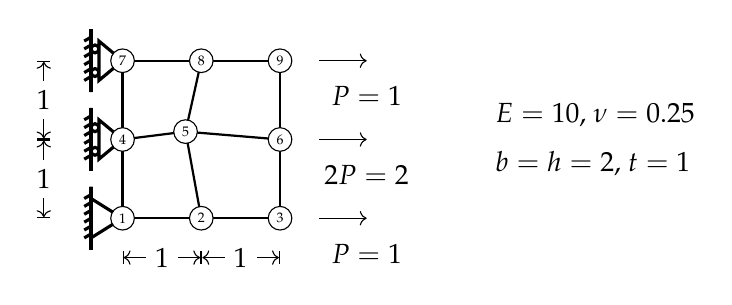
\begin{tikzpicture}[scale=1]
\coordinate(N1)at(0,0);
\coordinate(N2)at(1,0);
\coordinate(N3)at(2,0);
\coordinate(N4)at(0,1);
\coordinate(N5)at(.8,1.1);
\coordinate(N6)at(2,1);
\coordinate(N7)at(0,2);
\coordinate(N8)at(1,2);
\coordinate(N9)at(2,2);
\draw[thick](N1)--(N2)--(N3)--(N6)--(N9)--(N8)--(N7)--(N4)--cycle;
\draw[thick](N2)--(N5)--(N8);
\draw[thick](N4)--(N5)--(N6);
\HingeSupport[-90]{N1};
\RollerSupport[-90]{N4};
\RollerSupport[-90]{N7};
\begin{scope}[every node/.style={fill=white,circle,draw,inner sep=0,minimum size=3mm}]
\node at(N1){\tiny1};
\node at(N2){\tiny2};
\node at(N3){\tiny3};
\node at(N4){\tiny4};
\node at(N5){\tiny5};
\node at(N6){\tiny6};
\node at(N7){\tiny7};
\node at(N8){\tiny8};
\node at(N9){\tiny9};
\end{scope}
\draw[->](2.5,0)--++(.6,0)node[below=2mm]{$P=1$};
\draw[->](2.5,1)--++(.6,0)node[below=2mm]{$2P=2$};
\draw[->](2.5,2)--++(.6,0)node[below=2mm]{$P=1$};
\draw[|<->|](0,-.5)--++(1,0)node[midway,fill=white]{$1$};
\draw[|<->|](1,-.5)--++(1,0)node[midway,fill=white]{$1$};
\draw[|<->|](-1,0)--++(0,1)node[midway,fill=white]{$1$};
\draw[|<->|](-1,1)--++(0,1)node[midway,fill=white]{$1$};
\node[align=left]at(6,1){$E=10$, $\nu=0.25$\\[2mm]$b=h=2$, $t=1$};
\end{tikzpicture}
\caption{constant strain patch test}\label{fig:csmq_patch}
\end{figure}
The linear displacement field can be successfully computed by using CSMQ4 elements with arbitrary location of the middle node.

Since strain field remains constant, no couple stress would be generated in this example. As the result, whether nodal rotations are constrained has no impact on final results. Due to the same reason, any positive numbers can be chosen as the characteristic length $l$.
\section{Conclusions}
In this work, based on the consistent couple stress theory, a mixed variational theorem is developed with six independent fields. Finite elements of various types can be formulated accordingly for problems with both linear and nonlienar materials, although it is still difficult to further investigate the performance of the couple stress theory beyond elasticity for the moment, given that most existing constitutive models are developed based on the Cauchy theory. It would be interesting to see work in that regard in future.

The proposed elements have been implemented in \texttt{suanPan} \citep{Chang2021}. Sample model scripts can be found online\footnote{Link to the repository would be added after acceptance}.
\bibliography{S}
\end{document}